\documentclass[aspectratio=169,12pt]{beamer}
\usepackage{amsmath}
\usepackage{amssymb}
\usepackage[most]{tcolorbox}
\usepackage{tikz}
\usepackage{graphicx}
\usepackage[sfdefault,lf]{FiraSans}
\renewcommand{\familydefault}{\sfdefault}
\setlength{\parindent}{0pt}
\everymath{\displaystyle}

\setbeamertemplate{navigation symbols}{}
\setbeamertemplate{footline}{}
\setbeamertemplate{headline}{}

\definecolor{mmpageWhite}{HTML}{FCFBF7}
\definecolor{mmtanSoft}{HTML}{F7F5EF}
\definecolor{mmgreenDeep}{HTML}{244B2C}
\definecolor{mmgreenLeaf}{HTML}{5D8A56}
\definecolor{mmgreenSoft}{HTML}{E4EFD9}
\definecolor{mmtext}{HTML}{163221}

\setbeamercolor{background canvas}{bg=mmpageWhite}
\setbeamercolor{normal text}{fg=mmtext,bg=mmpageWhite}

\newtcolorbox{MMProblemCard}[1][]{enhanced,breakable=false,colback=white,colframe=black,boxrule=1.0pt,arc=5pt,left=3pt,right=3pt,top=2pt,bottom=2pt,before skip=0pt,after skip=0pt,height=0.26\textheight,valign=top,#1}
\newcommand{\KoruIcon}{\raisebox{-0.2em}{
\includegraphics[height=1.05em]{../../SITE/header-logo.png}}}
\newcommand{\HoeIcon}{\raisebox{-0.2em}{
\includegraphics[height=1.05em]{../../SITE/hoe.png}}}
\newcommand{\ScaffoldIcons}[1]{\ifcase#1\or \HoeIcon\or \HoeIcon\hspace{0.22em}\KoruIcon\or \KoruIcon\hspace{0.22em}\KoruIcon\hspace{0.22em}\KoruIcon\fi}
\newcommand{\WorksheetTitle}[2]{%
  {\colorbox{mmtanSoft}{\parbox[c][2.0em][c]{0.975\linewidth}{%
    \hspace{0.25em}{\Large\bfseries\textcolor{mmgreenDeep}{#1}\hfill\ScaffoldIcons{#2}}}}
  \par\vspace{0.08em}{\color{mmgreenLeaf}\rule{\linewidth}{2.0pt}}\par\vspace{0.04em}}
}
\newcommand{\MMProblem}[2]{\begin{MMProblemCard}\raggedright\small\textbf{#1.} #2\par\end{MMProblemCard}}

\setbeamertemplate{background}{
 \begin{tikzpicture}[remember picture,overlay]
 \draw[black,line width=1.5pt,rounded corners=10pt]
 ([xshift=0.45cm,yshift=-0.45cm]current page.north west)
 rectangle
 ([xshift=-0.45cm,yshift=0.45cm]current page.south east);
 \end{tikzpicture}
}

% Default worksheet generation rules:
% use notes-style beamer pages
% use bordered cards for individual problems
% target 9 problems per frame in a 3x3 grid
% target 3 frames per scaffold by default where content allows

\begin{document}\begin{frame}[t]
\WorksheetTitle{Start Tasks}
\vspace{-0.18em}
\begin{columns}[T,onlytextwidth]
\begin{column}{0.32\textwidth}\MMProblem{1}{Describe the box-and-whisker graph using CSSI.\\[0.4em]
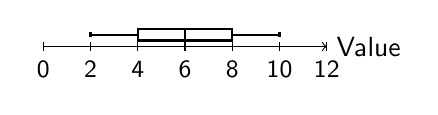
\begin{tikzpicture}[x=0.3cm,y=0.3cm,baseline=(current bounding box.center)]
  % axis
  \draw[->] (0,0) -- (12,0) node[right] {Value};
  \foreach \x in {0,2,4,6,8,10,12} \draw (\x,0.2) -- (\x,-0.2) node[below] {\small \x};
  % boxplot at y=0.5
  \draw[thick] (2,0.5) -- (4,0.5); % lower whisker
  \draw[thick] (4,0.25) rectangle (8,0.75); % box
  \draw[thick] (6,0.25) -- (6,0.75); % median line
  \draw[thick] (8,0.5) -- (10,0.5); % upper whisker
  \draw[thick] (2,0.4) -- (2,0.6); % min tick
  \draw[thick] (10,0.4) -- (10,0.6); % max tick
\end{tikzpicture}}\end{column}
\begin{column}{0.32\textwidth}\MMProblem{2}{Describe the box-and-whisker graph using CSSI.\\[0.4em]
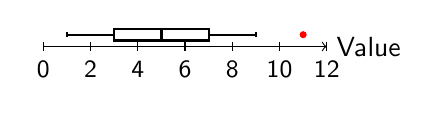
\begin{tikzpicture}[x=0.3cm,y=0.3cm,baseline=(current bounding box.center)]
  \draw[->] (0,0) -- (12,0) node[right] {Value};
  \foreach \x in {0,2,4,6,8,10,12} \draw (\x,0.2) -- (\x,-0.2) node[below] {\small \x};
  % boxplot with outliers
  \draw[thick] (1,0.5) -- (3,0.5);
  \draw[thick] (3,0.25) rectangle (7,0.75);
  \draw[thick] (5,0.25) -- (5,0.75);
  \draw[thick] (7,0.5) -- (9,0.5);
  \draw[thick] (1,0.4) -- (1,0.6);
  \draw[thick] (9,0.4) -- (9,0.6);
  % outlier at 11
  \fill[red] (11,0.5) circle (0.15);
\end{tikzpicture}}\end{column}
\begin{column}{0.32\textwidth}\MMProblem{3}{Describe the box-and-whisker graph using CSSI.\\[0.4em]
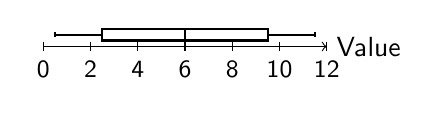
\begin{tikzpicture}[x=0.3cm,y=0.3cm,baseline=(current bounding box.center)]
  \draw[->] (0,0) -- (12,0) node[right] {Value};
  \foreach \x in {0,2,4,6,8,10,12} \draw (\x,0.2) -- (\x,-0.2) node[below] {\small \x};
  % boxplot with larger spread
  \draw[thick] (0.5,0.5) -- (2.5,0.5);
  \draw[thick] (2.5,0.25) rectangle (9.5,0.75);
  \draw[thick] (6,0.25) -- (6,0.75);
  \draw[thick] (9.5,0.5) -- (11.5,0.5);
  \draw[thick] (0.5,0.4) -- (0.5,0.6);
  \draw[thick] (11.5,0.4) -- (11.5,0.6);
\end{tikzpicture}}\end{column}
\end{columns}
\vspace{0.45em}
\begin{columns}[T,onlytextwidth]
\begin{column}{0.32\textwidth}\MMProblem{4}{Identify the Centre (median) for each boxplot above.}\end{column}
\begin{column}{0.32\textwidth}\MMProblem{5}{Identify the Shape (skewness) for each boxplot above.}\end{column}
\begin{column}{0.32\textwidth}\MMProblem{6}{Identify the Spread (IQR, range) for each boxplot above.}\end{column}
\end{columns}
\vspace{0.45em}
\begin{columns}[T,onlytextwidth]
\begin{column}{0.32\textwidth}\MMProblem{7}{Identify any Interesting features (outliers, groups) for each boxplot above.}\end{column}
\begin{column}{0.32\textwidth}\MMProblem{8}{What does CSSI stand for?}\end{column}
\begin{column}{0.32\textwidth}\MMProblem{9}{Match each letter of CSSI with its meaning.}\end{column}
\end{columns}
\end{frame}
\begin{frame}[t]
\WorksheetTitle{Start Tasks}
\vspace{-0.18em}
\begin{columns}[T,onlytextwidth]
\begin{column}{0.32\textwidth}\MMProblem{1}{Given a box-and-whisker graph with a median around 6 and IQR from 4 to 8, describe the centre and spread.}\end{column}
\begin{column}{0.32\textwidth}\MMProblem{2}{Given a box-and-whisker graph with a long upper whisker, describe the shape.}\end{column}
\begin{column}{0.32\textwidth}\MMProblem{3}{Given a box-and-whisker graph with an outlier at 12, describe the interesting feature.}\end{column}
\end{columns}
\vspace{0.45em}
\begin{columns}[T,onlytextwidth]
\begin{column}{0.32\textwidth}\MMProblem{4}{}\end{column}
\begin{column}{0.32\textwidth}\MMProblem{5}{}\end{column}
\begin{column}{0.32\textwidth}\MMProblem{6}{}\end{column}
\end{columns}
\vspace{0.45em}
\begin{columns}[T,onlytextwidth]
\begin{column}{0.32\textwidth}\MMProblem{7}{}\end{column}
\begin{column}{0.32\textwidth}\MMProblem{8}{}\end{column}
\begin{column}{0.32\textwidth}\MMProblem{9}{}\end{column}
\end{columns}
\end{frame}
\end{document}
